\documentclass[crop, tikz]{standalone}

\usepackage[utf8]{inputenc}
% 'crop' is the default for v1.0, before it was 'preview'
%\usetikzlibrary{...}% tikz package already loaded by 'tikz' option

\usetikzlibrary{arrows}
\usetikzlibrary{decorations.markings}
\usetikzlibrary{patterns}
\usetikzlibrary{calc}

%hexagon drawing variables
\def\ly{0.866025} %sin(pi/3) = sqrt(3)/2
\def\lx{0.5} %cos(pi/3) = 0.5
\def\hexSize{5} %size of the hexagon that'll be the extent of the fibre cross section
\def\coreSize{0.2} %size of hollow cores
\def\coreSep{0.5} %separation between core CENTRES HORIZONTALLY
\def\coreSepHeight{0.4464} %separation between core CENTRES VERTICALLY

\newcommand{\hexagon}[4]{
\begin{scope}[shift={#2}]
	\draw[#3, fill=#4] (-#1*\lx, #1*\ly) -- (#1*\lx, #1*\ly) -- (#1,0) -- (#1*\lx, -#1*\ly) -- (-#1*\lx, -#1*\ly) -- (-#1,0) -- cycle;
\end{scope}
} %\hexagon{centre-to-corner-length}{shift (x,y)}{line spec}{fill colour} [none is allowed for fillcolour]

\begin{document}
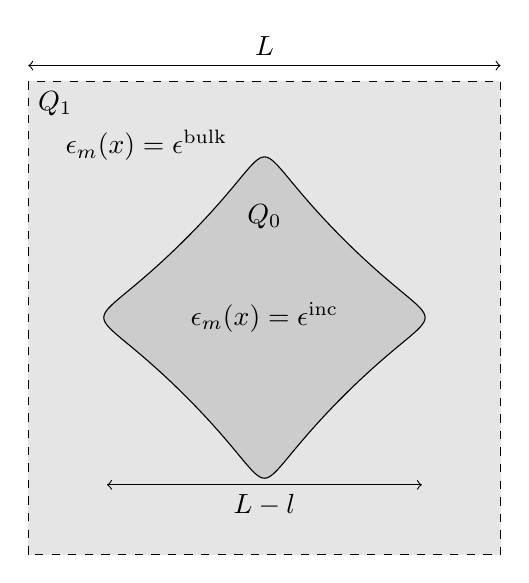
\begin{tikzpicture}[]
	

	% period cell boundary, weird start b/c of tikz cutoff behaviour
	\filldraw[black!10!white, draw=black, dashed] (0,-0.01) rectangle (6,6);

	% draw inclusion, label parts of the domain
	\filldraw[black!20!white, draw=black] plot [smooth cycle, tension=2.5] coordinates {(2,2) (4,2) (4,4) (2,4)};
	\node[anchor=north west] at (0,6) {$Q_1$};
	\node[anchor=south] at (3,4) {$Q_0$};

	% indicate length scales
	% period cell size
	\draw[<->] (0,6.2) -- (6,6.2); \node[anchor=south] at (3,6.2) {$L$};
	% inclusion size
	\draw[<->] (1,0.875) -- (5.0,0.875); \node[anchor=north] at (3.0,0.875) {$L-l$};
	% draw example material params: go for soft inclusion (a(x)=a) inside stiff matrix (a(x)=1)
	\node[anchor=center, align=center] at (3,3) {$\epsilon_m(x)=\epsilon^{\mathrm{inc}}$}; %\\ $\mu_m(x)=\mu^{\mathrm{inc}}$};
	\node[anchor=north, align=center] at (1.5,5.5) {$\epsilon_m(x)=\epsilon^{\mathrm{bulk}}$}; %\\ $\mu_m(x)=\mu^{\mathrm{bulk}}$};

\end{tikzpicture}
\end{document}